\documentclass[final]{cvpr}

\usepackage{times}
\usepackage{epsfig}
\usepackage{graphicx}
\usepackage{amsmath}
\usepackage{amssymb}

% Include other packages here, before hyperref.
\usepackage{acro}
\usepackage{csquotes}
\usepackage{mathtools}
\usepackage[ruled]{algorithm2e}

% If you comment hyperref and then uncomment it, you should delete
% egpaper.aux before re-running latex.  (Or just hit 'q' on the first latex
% run, let it finish, and you should be clear).
\usepackage[pagebackref=true,breaklinks=true,colorlinks,bookmarks=false]{hyperref}


\def\cvprPaperID{****} % *** Enter the CVPR Paper ID here
\def\confYear{2021}

\newcommand{\q}[1]{\enquote{#1}}
\newcommand{\Par}[1]{\left(#1\right)}
\newcommand{\Brac}[1]{\left[#1\right]}
\newcommand{\Set}[1]{\left\{#1\right\}}
\DeclarePairedDelimiter{\abs}{|}{|}
\DeclarePairedDelimiter{\norm}{\lVert}{\rVert}

\newcommand{\acdef}[2]{
	\DeclareAcronym{#1}{
		short = #1,
		long = #2,
	}
}
\acdef{RMSE}{root mean squared error}
\acdef{KNN}{$k$-nearest neighbours}
\acdef{SVD}{singular value decomposition}
\acdef{NCF}{neural collaborative filtering}
\acdef{CF}{collaborative filtering}
\acdef{SGD}{stochastic gradient descent}


\begin{document}

\title{
	Project report \\~\\
	\large{Team name: M2 Robo}
}

\author{
	Lee Chun Yin\\
	3035469140\\
	\and
	Chiu Yu Ying\\
	3035477630
	\and
	Chan Kwan Yin\\
	3035466978 \\
	Team leader
}

\maketitle

\clearpage

\section{Introduction}
\subsection{\ac{CF}}
\ac{CF} is a technique for recommendation system,
in which historical feedback data are used to infer connections between users and products~\cite{FactorMeet}.
While additional features can be introduced to offset certain bias effects~\cite{BellKor2008},
two inputs (user and product) and one output (user rating on the product) are generally sufficient
to train a \ac{CF} model without involving domain-specific data.

Two major approaches for \ac{CF} include neighbourhood models and latent factor models.
Neighbourhood models compare the similarity between users
and recommend products positively rated by similar users,
while latent factor models perform dimensional reduction on both users and movies
to a common, smaller set of feature attributes such that
users are recommended with movies of more coherent features.

\subsection{The Netflix Prize dataset}
The Netflix Prize is a competition for the prediction of users' favour of movies.
The dataset provides existing ratings of users on given movies,
and models are trained to predict new ratings.

\subsubsection{Dataset format}

The dataset contains 100480507 rows of data structured in the following format:

\begin{tabular}{|c|c|c|c|}
	\hline
	User ID & 490189 discrete values \\ \hline
	Movie ID & 17770 discrete values \\ \hline
	Rating & 1, 2, 3, 4, 5 \\ \hline
	Date & Dates from 1999 to 2005 \\ \hline
\end{tabular}

\subsubsection{Distribution of ratings}
Ratings are mostly distributed around 3 and 4,
as shown in Figure \ref{fig:rating-freq}.

Except for some extreme cases, the number of ratings per user over the 7 years
mostly follow an exponential relation for users from 10 to 1000 ratings,
as shown in Figure \ref{fig:user-rating-freq}.
The top 10 users with the highest number of ratings
range from 17651 to 8877.

For movies with at least 100 ratings (which is the case for the majority),
their numbers of ratings demonstrate a similar but more concave relationship,
as shown in Figure \ref{fig:movie-rating-freq}.

\begin{figure}
	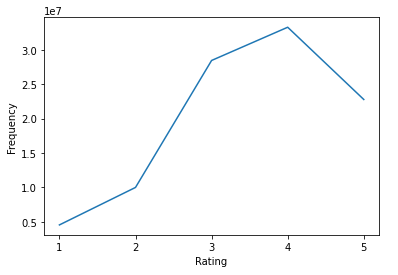
\includegraphics[width=0.5\textwidth]{screenshot20210422222105.png}
	\caption{Frequency of ratings}
	\label{fig:rating-freq}
\end{figure}

\begin{figure}
	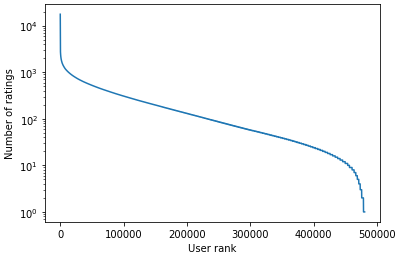
\includegraphics[width=0.5\textwidth]{screenshot20210422222340.png}
	\caption{Number of ratings per user}
	\label{fig:user-rating-freq}
\end{figure}

\begin{figure}
	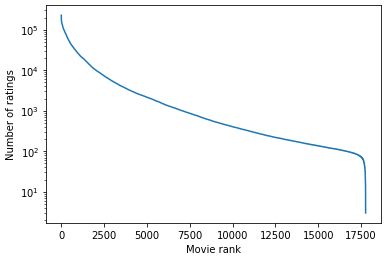
\includegraphics[width=0.5\textwidth]{screenshot20210422223229.png}
	\caption{Number of ratings per movie}
	\label{fig:movie-rating-freq}
\end{figure}

\subsubsection{Evaluation process}
To evaluate performance, 1425333 rows (about 1.42\% of all data) are speified as the standard "probe".
We perform analysis in the following procedure:

\begin{enumerate}
	\item Train the model with the 99055174 non-probe rows.
	\item Predict user ratings with the 1425333 probe rows.
	\item Compute the \ac{RMSE} between the predicted data and actual data.
    $$ \text{RMSE} = \sqrt{\sum_{(i, j) \in E} \frac{{(\hat r_{ij} - r_{ij})}^2}{\left| E \right|}} $$
where $E$ is the set of retained evaluation data.
\end{enumerate}


In this project, we evaluate three models, namely:

\begin{itemize}
	\item \ac{KNN}, a simple neighbourhood model
	\item \ac{SVD}, a latent factor model that accounts for user bias
	\item \ac{NCF}, a latent factor model that represents features with neural network weights
\end{itemize}

Originally, we proposed three models KNN, SVD and SVD++ (a SVD model with time features).
Due to the high similarity between SVD and SVD++,
we proposed the use of NCF instead,
while the additional time effect bias in SVD++ is left out as a to-do.

\subsection{Notations}
In this report, we denote variables about the dataset as follows:
\begin{itemize}
	\item $m$: number of users
	\item $n$: number of movies
	\item $N$: number of ratings
	\item $r_{ij}$: rating of user $i$ on movie $j$
\end{itemize}

\section{Data preprocessing}
Due to performance issues with CSV parsing, we wrote a separate program `preprocess-dataset`,
which reformats the input files into a numpy saved array
which contains the following columns derived from the original dataset:

\begin{itemize}
	\item User ID
	\item Movie ID
	\item Rating value
	\item Year of rating
	\item Day of year of rating
	\item Day of week of rating
	\item Whether the rating is probed data
\end{itemize}

During runtime, the data are represented in \ac{CSR} format
for a sparse $m \times n$ matrix.

\section{\ac{KNN}}
\ac{KNN} is an example of neighbourhood models.
It seeks to provide recommendations based on the behaviour of similar users.
In \ac{KNN} model, we assume that similar users will give close ratings on similar movies.
To predict the rating $\hat r_{ij}$ of user $i$ on movie $j$ ($1 \le i \le m, 2 \le j \le n$),
the $k$ most similar users ($n_1, \ldots, n_k$) to user $i$ are computed based on similar choices of ratings,
and $\hat r_{ij}$ is estimated based on the known values $r_{n_1j}, \ldots, r_{n_kj}$.

\subsection{Algorithm}
The training algorithm involves the following steps:

The algorithm first finds $q$, the set of $q$ users with the highest number of ratings.
The distance $d(i, j)$ for $i \in [1, m], j \in q \setminus \Set{i}$ is then computed,
and the neighbourhood $K_i \subset q$ of each user $i$ is evaluated as the $k$ users with the lowest distance.
The prediction of the rating $r_{ij}$ is computed by
aggregating the neighbourhood ratings with $A(\Set{r_{xj} : x \in K_i})$.
The memory complexity of these operations (except $d$ and $A$) is $O(qn)$.

In this KNN implementation, there are four hyperparameters to be considered, namely neighbourhood size $k$, neighbourhood candidate size $q$, distance function $d$ and aggregation function $A$.

\subsubsection{Neighbourhood size $k$}
$k$ refers to the number of nearest neighbours to be included in recommendation system. 

A large value of $k$ would reduce accuracy as users with lower similarity are selected.
On the other hand, a small value of $k$ would be biased over the choice of the most similar user.
We have tested with different values of $k$ with different values of the other hyperparameters.

As a baseline model, we also set $k=m$, i.e.
to evaluate the RMSE by taking the plain arithmetic mean of all users.

\subsubsection{Neighbourhood candidate size $q$}
$q$ means the number of neighbour candidate the recommendation system considered. 
We tried different values of $q$, which led to different sets of k-nearest neighbours being selected each time.

\subsubsection{Distance function $d$}
The distance function $d: \mathbb R^n \times \mathbb R^n \to [0, 1]$
observes the deviation in interests between two different users.
$d(i, j) = 0$ iff $i = j$, and $d(i, j) = d(j, i) \forall i = j$.
Although $d(i, j) < d(i, k)$ implies that $j$ is more similar to $i$ than $k$ is,
it is not necessary that $d$ follows triangular inequality.


\paragraph{Cosine}
The cosine distance is defined as
$$ d(\mathbf x, \mathbf y) = 2 \frac
{\Par{\mathbf x - \mathbf b} \cdot \Par{\mathbf y - \mathbf b}}
{\norm{\mathbf x - \mathbf b} \norm{\mathbf y - \mathbf b}} - 1 $$
where $\mathbf b = \frac1n \sum_{i=1}^m \mathbf r_{i\cdot}$,
i.e. the mean rating of each movie.
This metric emphasizes the difference between users who gave ratings better or worse than the average,
e.g. the difference between $3$ and $5$ is more important than the difference between $1$ and $3$
when the average rating is $4$.
It can be thought of a metric to determine how "abnormal" a user is.
The multiplier is to correct the distance range to $[0, 1]$.

\paragraph{$p$-norm}
The $p$-norm distance is defined as the $p$-norm of two vectors
normalized by the maximum possible distance, i.e.
$$ d(\mathbf x, \mathbf y) = \frac
{\Par{\sum_{i=1}^n \abs{x_i - y_i}^p}^{1/p}}
{4 n^{1/p}} $$.

\subsubsection{Aggregation function $A$}
We computed both baseline and average aggregation functions. 

\subsection{Findings}

\subsubsection{Baseline model result}
The RMSE value attained in baseline model is $1.0528$.


\subsubsection{Cosine distance model result}
\begin{figure}[h]
	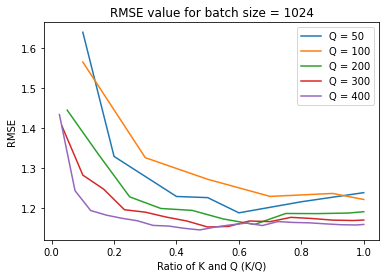
\includegraphics[width=0.5\textwidth]{knn-cosine-graph.png}
	\caption{RMSE for different combination of  q and k with cosine distance function}
	\label{fig:rmse-knn-QK}
\end{figure}

We can see the RMSE values decreased with the increasing q value in general.
The curve with $q = 400$ has the smallest values for nearly all ratio of $k$ and $q$.
The curve with $q = 50$ however has larger values for most of the ratio values than the curve with $q = 100$.
All the curves have non-smooth logarithmic curves with fluctuations between ratio = 0.1 to ratio = around 0.7. 
The lowest RMSE value attained with the cosine distance function is $1.1455$ with ratio = 0.475 ($q = 400$ and $k=190$).
For the other values of $q$, when $q = 300$, the lowest value found in ratio = 0.5 ($k = 150$).
When $q = 200$, the lowest value belonged to ratio = 0.65 ($k = 130$).
When $q = 100$, the lowest value attained at ratio = 1 ($k = 100$).
When $q = 50$, the lowest belonged to ratio = 0.6 ($k = 30$).
To conclude, the ratios for the lowest value of RMSE for each curves varied.




\section{\ac{SVD}}
\subsection{Background}

\subsubsection{Learning rate $\alpha$}
\subsubsection{Regularization $\lambda$}
\subsubsection{Rank of factorization $k$}
\subsubsection{Number of epochs $\xi$}
\subsubsection{Batch size $\beta$}

\subsection{Findings}


\section{\ac{NCF}}
\subsection{Background}

\subsection{Findings}


\section{Conclusion}

{\small
	\bibliographystyle{ieee_fullname}
	\bibliography{egbib}
}

\end{document}
